\newpage
\subsection{User Story 24:}
Workflow des demandes à l'administrateur.  Le workflow de l'administrateur doit être relativement
simple. Il se base sur quelque états :

\begin{itemize}
  \item pris en compte
  \item traité
  \item traité, disponible après redémarrage de l'application
  \item complément d'information
  \item rejeté
  \item clos
\end{itemize}


\begin{figure}[!h]
  \begin{center}
        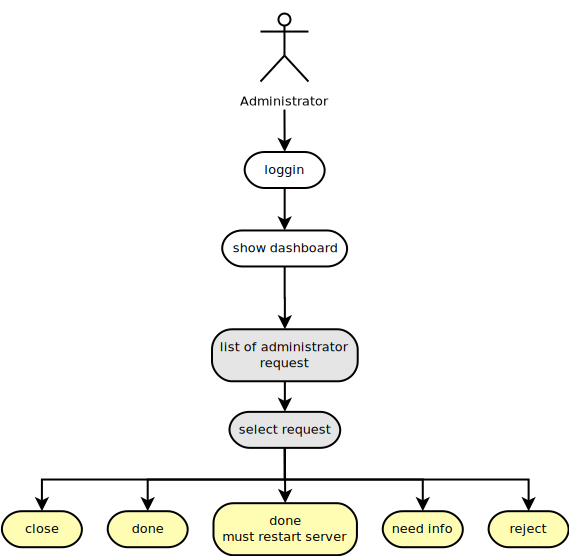
\includegraphics[width=0.7\textwidth]{US24}
        \label{US24-dia}
  \end{center}
\end{figure}